\documentclass[12pt]{article}
\usepackage[utf8]{inputenc}
\usepackage[russian]{babel}
\usepackage{amssymb}
\usepackage{authblk}
\usepackage{graphicx}
\title{2.1.3. Определение $\gamma$ по скорости звука в газе}
\author{Реутский Даниил, 793}
\begin{document}

\maketitle

\textbf{Цель:} измерение частоты колебаний и длины волны при резонансе звуковых колебаний в газе, заполняющем трубу; определение показателя адиабаты с помощью уравнения состояния идеального газа.

~

\textbf{Инструменты:} звуковой генератор; электронный осциллограф; микрофон; телефон; теплоизолированная труба, обогреваемая водой из термостата; баллон со сжатым воздухом; газгольдер;

~

\textbf{Введение.} Скорость звука в газе может быть найдена по формуле
%
$$c = \sqrt{\gamma \frac{RT}{\mu}},$$
%
где $\mu$ --- молярная масса газа. Выразим постоянную адиабаты:
$$\gamma = \frac{\mu}{RT} c^2.$$

Звуковые волны, проходя через трубу с газом, отражаются от стеноки накладываются друг на друга. Но если длины трубы кратна полуволне:
%
$$L = n \frac{\lambda}{2}~~~(n \in \mathbb{N}),$$
%
то отражённые волны совпадают по фазе. Они накладываются друг на друга, и наступает резонанс.

Зафиксируем длину трубы $L$. Будем генерировать звуковые волны частотой $f$. Допустим, при $f = f_0$ наступил резонанс. Тогда для этой частоты справедливо
$$L = \frac{\lambda_0}{2}n = \frac{c}{2f_0}n.$$

Если следующая найденная резонансная частота есть $f_1$, то
$$L = \frac{c}{2f_1}(n + 1).$$

Продожим эту последовательность:
$$L = \frac{c}{2f_k}(n + k)$$
$$f_k = \frac{c}{2L}n + \frac{c}{2L}k$$

Таким образом, зависимость $f(k)$ линейна, и коэффициент наклона графика в осях $k$ и $f$ будет равен $c/2L$.

~

\textbf{Экспериментальная установка.} Представляет из себя трубу, в одном конце которой установлен телефон, возбуждающий звуковые колебания, а в другом  микрофон, улавливающий их. Источник колебаний телефона --- подключенный к нему звуковой генератор. Микрофон подключен ко входу осциллографа, его сигнал можно наблюдать на экране. Труба нагревается до определённой температуры водой из термостата. Для каждой температуры проводятся измерения для определения скорости звука.

\begin{center}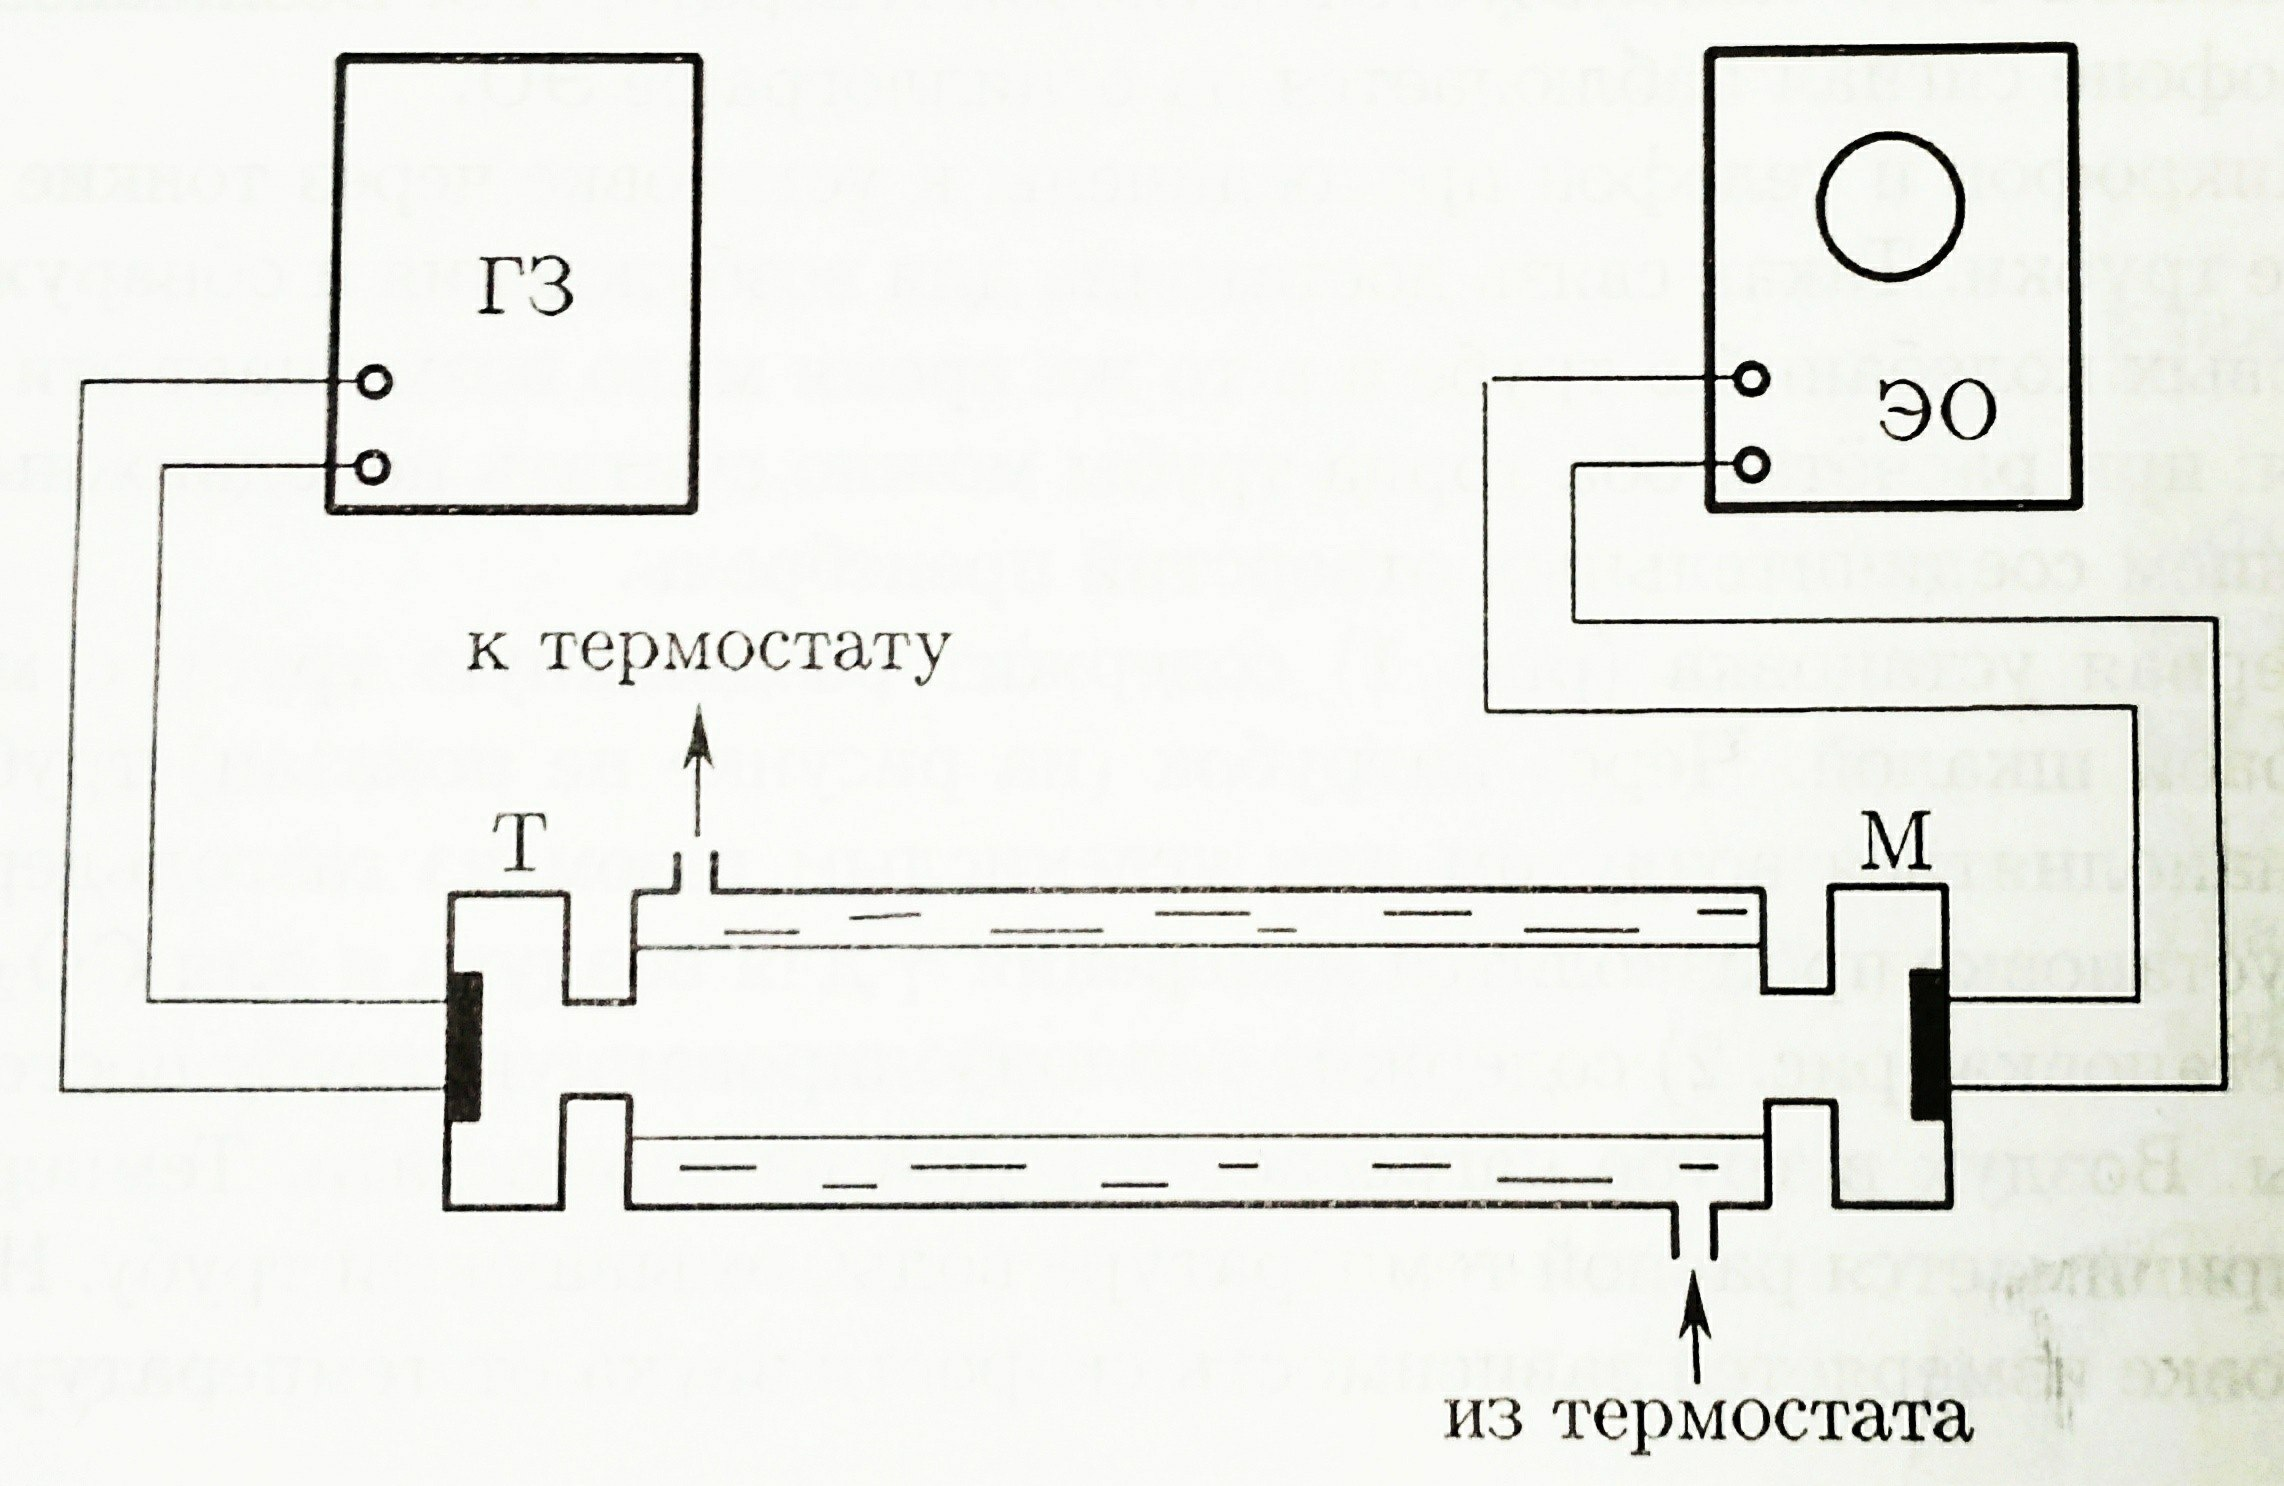
\includegraphics[width=0.7\textwidth]{2131.jpg}\end{center}
\newpage
\textbf{Экспериментальные данные.}

~

\noindent\begin{tabular}{ |l|l|l|l|l|l|l|l|l| }
  \hline
  ~ & $t = 25^\circ$ & $t = 30^\circ$ & $t = 35^\circ$ & $t = 40^\circ$ & $t = 45^\circ$ & $t = 50^\circ$ & $t = 55^\circ$ & $t = 60^\circ$ \\
  \hline
$k$ & $f$, Гц & $f$, Гц & $f$, Гц & $f$, Гц & $f$, Гц & $f$, Гц & $f$, Гц & $f$, Гц \\
\hline
1 & 473 & 482 & 488 & 488 & 494 & 499 & 503 & 506 \\
2 & 699 & 710 & 716 & 722 & 728 & 732 & 738 & 746 \\
3 & 926 & 941 & 948 & 957 & 963 & 971 & 980 & 987 \\
4 & 1153 & 1173 & 1181 & 1193 & 1202 & 1211 & 1220 & 1228 \\
5 & 1384 & 1407 & 1417 & 1431 & 1442 & 1453 & 1464 & 1474 \\
6 & 1612 & 1640 & 1653 & 1668 & 1679 & 1694 & 1706 & 1718 \\
7 & 1843 & 1873 & 1890 & 1904 & 1920 & 1935 & 1950 & 1964 \\
8 & 2073 & 2108 & 2124 & 2143 & 2159 & 2178 & 2191 & 2209 \\
9 & 2303 & 2341 & 2363 & 2380 & 2398 & 2418 & 2436 & 2455 \\
\hline
\end{tabular}

~

\begin{center}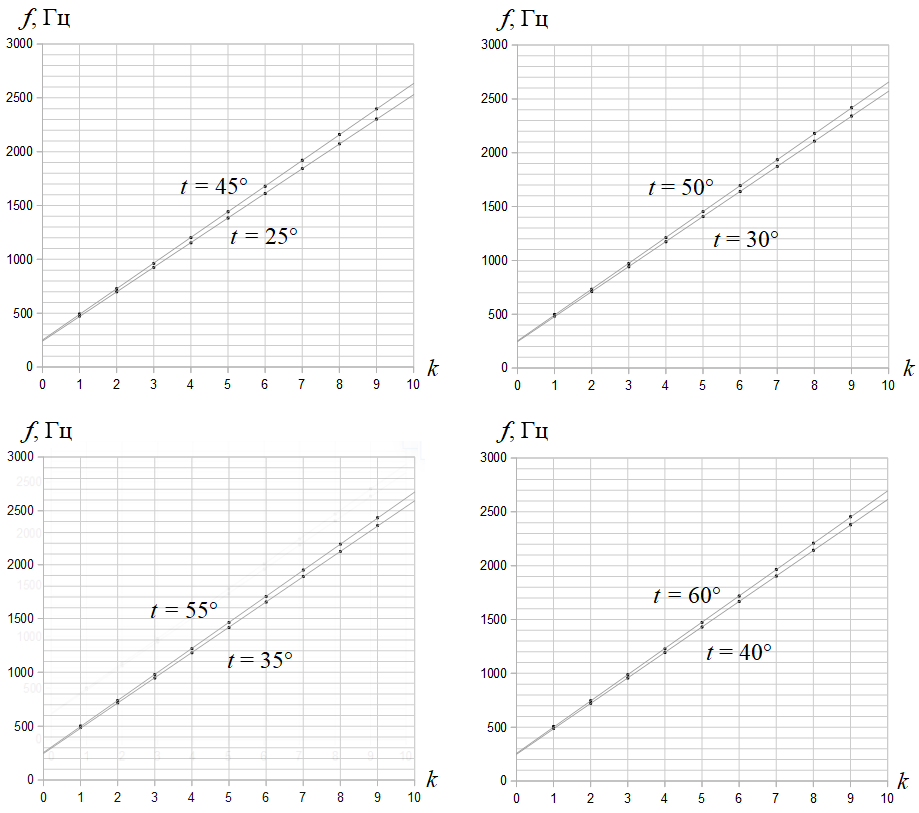
\includegraphics[width=1\textwidth]{2132.png}\end{center}
\newpage
Для каждой температуры находим $\alpha = c/2L$ методом наименьших квадратов.

$\langle k \rangle = 5, \langle k^2 \rangle \approx 31,666$

~

\noindent\begin{tabular}{ |l|l|l|l|l|l|l|l|l| }
  \hline
  $t$ & $25^\circ$ & $30^\circ$ & $35^\circ$ & $40^\circ$ & $45^\circ$ & $50^\circ$ & $55^\circ$ & $60^\circ$ \\
\hline
$\langle f \rangle$, Гц & 1385 & 1408 & 1420 & 1431 & 1442 & 1454 & 1465 & 1476\\
$\langle f^2 \rangle$, кГц$^2$ & 2,267 & 2,344 & 2,383 & 2,423 & 2,460 & 2,501 & 2,537 & 2,575\\
$\langle kf \rangle$, Гц & 8451 & 8592 & 8664 & 8736 & 8802 & 8875 & 8939 & 9007\\
$\alpha$, Гц & 228,9 & 232,6 & 234,6 & 236,67 & 238,3 & 240,4 & 241,9 & 243,8\\
$\sigma_\alpha$, Гц & 0,3 & 0,3 & 0,4 & 0,19 & 0,3 & 0,4 & 0,3 & 0,4\\
\hline
\end{tabular}

~

Использованные выражения для $\alpha$ и $\sigma_\alpha$:
$$\alpha = \frac{\langle kf \rangle - \langle k \rangle \langle f \rangle}{\langle k^2 \rangle - \langle k \rangle ^2}$$

$$\sigma_\alpha = \frac{1}{\sqrt{n}} \sqrt{\frac{\langle f^2 \rangle - \langle f \rangle ^2}{\langle k^2 \rangle - \langle k \rangle ^2} - \alpha^2}$$

То же, но вместо букв подставлены цифры, и так 8 раз (размерность подразумевается):
$$t = 25^\circ:~~~\alpha = \frac{ 8451  -  5.0 \cdot 1385 }{ 31.66  -  5.0  ^2},~~~\sigma_\alpha = \frac{1}{\sqrt{9}} \sqrt{\frac{ 2267889  -  1385  ^2}{ 31.66  -  5.0  ^2} - 228.9^2}$$

$$t = 30^\circ:~~~\alpha = \frac{ 8592  -  5.0 \cdot 1408 }{ 31.66  -  5.0  ^2},~~~\sigma_\alpha = \frac{1}{\sqrt{9}} \sqrt{\frac{ 2344350  -  1408  ^2}{ 31.66  -  5.0  ^2} - 232.6^2}$$

$$t = 35^\circ:~~~\alpha = \frac{ 8664  -  5.0 \cdot 1420 }{ 31.66  -  5.0  ^2},~~~\sigma_\alpha = \frac{1}{\sqrt{9}} \sqrt{\frac{ 2383534  -  1420  ^2}{ 31.66  -  5.0  ^2} - 234.6^2}$$

$$t = 40^\circ:~~~\alpha = \frac{ 8736  -  5.0 \cdot 1431 }{ 31.66  -  5.0  ^2},~~~\sigma_\alpha = \frac{1}{\sqrt{9}} \sqrt{\frac{ 2423397  -  1431  ^2}{ 31.66  -  5.0  ^2} - 236.6^2}$$

$$t = 45^\circ:~~~\alpha = \frac{ 8802  -  5.0 \cdot 1442 }{ 31.66  -  5.0  ^2},~~~\sigma_\alpha = \frac{1}{\sqrt{9}} \sqrt{\frac{ 2460298  -  1442  ^2}{ 31.66  -  5.0  ^2} - 238.3^2}$$

$$t = 50^\circ:~~~\alpha = \frac{ 8875  -  5.0 \cdot 1454 }{ 31.66  -  5.0  ^2},~~~\sigma_\alpha = \frac{1}{\sqrt{9}} \sqrt{\frac{ 2501073  -  1454  ^2}{ 31.66  -  5.0  ^2} - 240.4^2}$$

$$t = 55^\circ:~~~\alpha = \frac{ 8939  -  5.0 \cdot 1465 }{ 31.66  -  5.0  ^2},~~~\sigma_\alpha = \frac{1}{\sqrt{9}} \sqrt{\frac{ 2537473  -  1465  ^2}{ 31.66  -  5.0  ^2} - 241.9^2}$$

$$t = 60^\circ:~~~\alpha = \frac{ 9007  -  5.0 \cdot 1476 }{ 31.66  -  5.0  ^2},~~~\sigma_\alpha = \frac{1}{\sqrt{9}} \sqrt{\frac{ 2575878  -  1476  ^2}{ 31.66  -  5.0  ^2} - 243.8^2}$$

Скорость звука и её погрешность вычисляются соответственно по формулам:

$$c = 2\alpha L,~~~\sigma_c = c \sqrt{(\frac{\sigma_\alpha}{\alpha})^2 + (\frac{\sigma_L}{L})^2}$$

Подставим в эти формулы $\alpha$ и $\sigma_\alpha$ для каждой температуры:

~

\noindent\begin{tabular}{l@{~~~}l}
$t = 25^\circ:$ & $c = 2 \cdot 0.74 \cdot 228.9$ м/с $=338.7$ м/с \\
~ & $\sigma_c = 338.7 \sqrt{(\frac{0.3}{228.9})^2 + (\frac{1}{740})^2}$ м/с $ = 0.6$ м/с \\
\end{tabular}

\noindent\begin{tabular}{l@{~~~}l}
$t = 30^\circ:$ & $c = 2 \cdot 0.74 \cdot 232.6$ м/с $=344.2$ м/с \\
~ & $\sigma_c = 344.2 \sqrt{(\frac{0.3}{232.6})^2 + (\frac{1}{740})^2}$ м/с $ = 0.6$ м/с \\
\end{tabular}

\noindent\begin{tabular}{l@{~~~}l}
$t = 35^\circ:$ & $c = 2 \cdot 0.74 \cdot 234.6$ м/с $=347.2$ м/с \\
~ & $\sigma_c = 347.2 \sqrt{(\frac{0.4}{234.6})^2 + (\frac{1}{740})^2}$ м/с $ = 0.7$ м/с \\
\end{tabular}

\noindent\begin{tabular}{l@{~~~}l}
$t = 40^\circ:$ & $c = 2 \cdot 0.74 \cdot 236.67$ м/с $=350.3$ м/с \\
~ & $\sigma_c = 350.3 \sqrt{(\frac{0.19}{236.67})^2 + (\frac{1}{740})^2}$ м/с $ = 0.5$ м/с \\
\end{tabular}

\noindent\begin{tabular}{l@{~~~}l}
$t = 45^\circ:$ & $c = 2 \cdot 0.74 \cdot 238.3$ м/с $=352.6$ м/с \\
~ & $\sigma_c = 352.6 \sqrt{(\frac{0.3}{238.6})^2 + (\frac{1}{740})^2}$ м/с $ = 0.7$ м/с \\
\end{tabular}

\noindent\begin{tabular}{l@{~~~}l}
$t = 50^\circ:$ & $c = 2 \cdot 0.74 \cdot 240.4$ м/с $=355.8$ м/с \\
~ & $\sigma_c = 355.8 \sqrt{(\frac{0.4}{240.4})^2 + (\frac{1}{740})^2}$ м/с $ = 0.7$ м/с \\
\end{tabular}

\noindent\begin{tabular}{l@{~~~}l}
$t = 55^\circ:$ & $c = 2 \cdot 0.74 \cdot 241.9$ м/с $=358.0$ м/с \\
~ & $\sigma_c = 358.0 \sqrt{(\frac{0.3}{241.9})^2 + (\frac{1}{740})^2}$ м/с $ = 0.7$ м/с \\
\end{tabular}

\noindent\begin{tabular}{l@{~~~}l}
$t = 60^\circ:$ & $c = 2 \cdot 0.74 \cdot 243.8$ м/с $=360.8$ м/с \\
~ & $\sigma_c = 360.8 \sqrt{(\frac{0.3}{243.8})^2 + (\frac{1}{740})^2}$ м/с $ = 0.8$ м/с \\
\end{tabular}

~

Поскольку
$$c^2 = \frac{\gamma R}{\mu} T,$$
\noindent то коэффициент при $T$ (назовём его $\beta$) может быть найден при помощи метода наименьших квадратов.

Составим для этого таблицу.

~

\noindent\begin{tabular}{|l|l|l|l|}
\hline
$t, ^\circ$C & $T,$ К & $c,$ м/с & $c^2,$ м$^2$/с$^2$ \\
\hline
25 & 298 & 338,7 & 114717 \\
30 & 303 & 344,2 & 118473 \\
35 & 308 & 347,2 & 120547 \\
40 & 313 & 350,3 & 122710 \\
45 & 318 & 352,6 & 124326 \\
50 & 323 & 355,8 & 126593 \\
55 & 328 & 358,0 & 128164 \\
60 & 333 & 360,8 & 130176 \\
\hline
\end{tabular}

~

Коэффициент $\beta$ и его погрешность $\sigma_\beta$ находим по формулам
$$\beta = \frac{\langle Tc^2 \rangle}{\langle T^2 \rangle},~~~\sigma_\beta = \frac{1}{\sqrt{n}} \sqrt{\frac{\langle c^4 \rangle}{\langle T^2 \rangle} - \beta^2}$$

Необходимые средние значения (размерность подразумевается):
$$\langle Tc^2 \rangle = 38929080,~~~
\langle T^2 \rangle = 99671,~~~
\langle c^4 \rangle = 123213$$

Подставляем их в формулы:
$$\beta = \frac{38929080}{99671} = 390,5,~~~\sigma_\beta = \frac{1}{\sqrt{8}} \sqrt{\frac{123213}{99671} - 390,5^2} = 0,7$$

А вот и график на следующей странице:

\begin{center}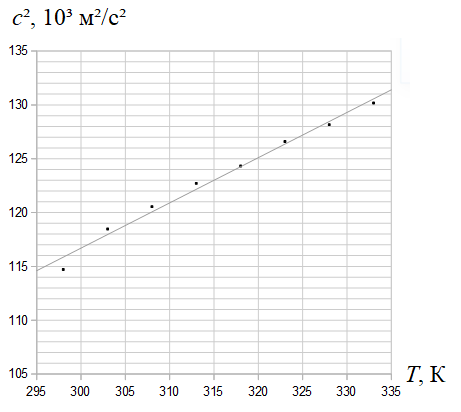
\includegraphics[width=0.7\textwidth]{2133.png}\end{center}

Обратите внимание, как располагаются точки относительно прямой. Это свидетельство того, что на больших диапазонах температуры зависимость вряд ли будет иметь линейный характер.

$\gamma$ и её погрешность находим из формул
$$\gamma = \frac{\beta \mu}{R},~~~\sigma_\gamma = \gamma\sqrt{(\frac{\sigma_\beta}{\beta})^2 + (\frac{\sigma_\mu}{\mu})^2}$$
$$\gamma = \frac{390,5 \cdot 0,029}{8,314472} = 1,36,~~~\sigma_\gamma = \gamma\sqrt{(\frac{0,7}{390,5})^2 + (\frac{1}{29})^2} = 0,05$$

Итак, мы нашли постоянную адиабаты для воздуха в одной теплоизолированной трубе:

$$\gamma = 1,36 \pm 0,05$$
\end{document}